\documentclass[11pt, letterpaper]{article}
\usepackage[margin=1in]{geometry}
\usepackage[utf8]{inputenc}
\usepackage[all]{xy}
\usepackage[hidelinks]{hyperref}
\usepackage{url, amsmath, amsfonts, stmaryrd, amssymb, amsthm, mathtools, enumerate, bm, geometry, tabularx, graphicx, caption}

\title{\textbf{Understanding Flight Delays}\\\textbf{CSE 519: Data Science Fundamentals}\\\textbf{Project Proposal}}
%\author{
%  Kai Li\\
%  \texttt{kai.li@stonybrook.edu}
%  \and
%  Peng Fei Yao\\
%  \texttt{pengfei.yao@stonybrook.edu}
%}
\date{Stony Brook University --- \today}

\begin{document}
\maketitle

\section{Introduction and Objectives}
Airline flight delay is one of the most severe problems across the globe in the 21st century. Between 2012 and 2019, the average delay rate for operating carrier flights is about 19.23\%, based on the Airline On-Time Statistics and Delay Causes data provided by the U.S. Department of Transportation (DOT) Bureau of Transportation Statistics (BTS) \cite{web:bts}. As the number of flight operations was generally increasing, the Federal Aviation Administration (FAA) handled more than 10 million passenger flights in 2019 with 2.9 million passengers flying every day in and out of United States airports \cite{web:faa1}. On the other hand, flight delay has been an issue for many years that can potentially become worse in the future if there is not a clear understanding of the causes and proper solution.

Flight delay releases pressure on everything related to aviation such as the National Airspace System (NAS), air traffic controllers, passengers, airlines, airports and the United States economy \cite{ar:carvalho_et_al, web:faa2, ar:peterson_neels_barczi_graham}. The NAS is a complicated network that controls air navigation facilities, airports, landing areas, aeronautical information, and so on \cite{web:faa3}. In particular, flight delay is one of the most pressing problems for the NAS operations and air traffic controllers because of the flexibility to adjust flight and airport schedules. Furthermore, from an economics perspective, flight delays result in the reduction of business productivity and active leisure for passengers to compensate for the additional air travel time \cite{ar:peterson_neels_barczi_graham}. What is more, passengers' preferences on airline carriers and airports can change due to flight delays, which can result in the jeopardization of airline companies' marketing strategies. Last but not least, the total estimated cost of flight delays in the United States has increased every year. FAA \cite{web:faa2} reported the total cost of delays separated into categories of airlines, passengers, lost demand and indirect costs, as shown in Table \ref{tab:cost}. 

\begin{table}[h!]
\centering
\begin{tabular}{lcccccccc}
             & 2012 & 2013 & 2014 & 2015 & 2016 & 2017 & 2018 & 2019 \\ 
\hline
 Airlines    & 5.7  & 6.0  & 5.8  & 5.8  & 5.6  & 6.4  & 7.7  & 8.3 \\  
 Passengers  & 9.7  & 11.0 & 10.5 & 13.3 & 13.3 & 14.8 & 16.4 & 18.1 \\
 Lost Demand & 1.3  & 1.4  & 1.4  & 1.8  & 1.8  & 2.0  & 2.2  & 2.4 \\
 Indirect    & 2.5  & 2.7  & 2.6  & 3.1  & 3.0  & 3.4  & 3.9  & 4.2 \\
\hline
 \textbf{Total} & \textbf{19.2} & \textbf{21.1} & \textbf{20.3} & \textbf{24.0} & \textbf{23.7} & \textbf{26.6} & \textbf{30.2} & \textbf{33.0}
\end{tabular}\caption{Total Cost of Flight Delay in the U.S. (in billion dollars)}\label{tab:cost}
\end{table}

The total cost of flight delay in the United States increased by 71.88\% between 2012 and 2019, with an average total cost increase of 8.30\% per year. Additionally, an interesting observation is that the largest increase in the total cost was the increase in the cost of delay to passengers. In a study measuring the econometric estimation of the welfare impact of flight delays, Britto et al. \cite{ar:britto_dresner_voltes} suggests that each passenger from the United States can gain about 1.50 to 2.50 dollars from a 10\% reduction in delays. Hence, the influence of flight delays is reinforced again.

The objectives of this project are to examine the impact of flight delays on airports and airlines and to model when flight delays are likely. In this project, we shall follow the general definition of "flight delay" and "on-time" according to the FAA, BTS, and NAS. That is, we consider a flight is delayed if the flight arrived at the airport gate 15 minutes or more after the scheduled arrival time as reflected in the Computerized Reservation System (CRS). Similarly, we consider a flight to be on-time if the flight arrived at the gate less than 15 minutes than the scheduled time appeared in the CRS. Besides this overview, Section \ref{sec:data_meth} of the proposal will discuss the data collection process and how we will perform the appropriate data analysis procedures to better understand flight delays. In Section \ref{sec:da_mp}, a more detailed plan will be provided on the data analysis and predictive modeling process so that we are ready to answer the proposed research questions. Finally, we will give some basic data descriptions with visualizations in Section \ref{sec:da}.

\section{Data and Methodology}\label{sec:data_meth}
The dataset used in this project comes from the BTS database called Airline On-Time Arrival Performance Data. BTS database is reliable because the data is open-sourced under the U.S. government. The data consists of essential variables, such as airline, airport, year and month, number of flights delayed due to weather, delayed arrivals in minutes, etc, to record on-time data for the commercial carrier network. We selected the period from January 2012 to December 2019. Besides the primary dataset, we also incorporated some secondary datasets with only one property (e.g. which airline carrier group) from the BTS database to further analyze questions of interest. Note that the secondary datasets need to be cleaned so that the corresponding subset of information can be merged into the primary dataset. For example, records before 2012 and after 2019 in the auxiliary data are deleted. After a series of data cleaning, the datasets will be merged based on the primary key(s) in the main dataset and proceed to further enrich the available data.

We will be using Python to perform all sorts of data manipulation, analysis, and modeling procedures. Here, we list some potentially useful packages. For data manipulation and scientific computing, we will use \texttt{pandas} and \texttt{NumPy}. Libraries such as \texttt{Matplotlib} and \texttt{seaborn} are excellent data visualization tools. Furthermore, \texttt{scikit-learn} and \texttt{SciPy} provide ample powerful methods to perform predictive data analysis and relevant statistical procedures.

\section{Data Analysis and Modeling Procedures}\label{sec:da_mp}
\subsection{Delays in Busiest Airports and the others}
The first research question considers the delay pattern difference between the busiest airports and less busy airports. To properly define which airports are busy, we follow the classification of major airports defined in the BTS Airline On-Time Statistics and Delay Causes dataset. There are 30 major airports, which are all the core international airports around the United States, out of 379 airports in our primary dataset. Therefore, we consider the major airports as the busiest airports among all the airports. We will perform a series of data analysis procedures to compare the delay percentage by year, month, airport, busiest vs. not the busiest, and so on both quantitatively and visually to answer the question.

\subsection{Delays Versus Airline Market Size}
We are also interested in how airlines with a different proportion of market revenues behave in front of delay rates. We will add two extra secondary datasets to solve the puzzle. One of the datasets divides the 23 airline companies in the primary dataset into different carrier groups, decoded by the BTS Aviation Support Tables database. In all the 23 airline carriers investigated, the carriers are either in group National Carriers (carriers with annual revenue over \$100 million to \$1 billion) or group Major Carriers (carriers with annual revenue over \$1 billion) after an appropriate cleaning to the duplicated values in the secondary dataset.

Another secondary dataset separates the airline carriers into marketing carriers and regular carriers. The marketing carrier group is a special subset of all airline carriers in that marketing carriers have market flights for themselves and also regional codeshare partners in some cases, as illustrated in the BTS Airline On-Time Performance Data database. We will apply similar analysis procedures to figure out the relationship between carrier group and flight delay.

\subsection{Delays versus Airline Establishment Time}
Some of the airline carriers established since 1960, such as the American Airline Inc. Some others are relatively new, such as JetBlue Airways started in 2000. Does the establishment time of airline companies affect the delay rate? We have a dataset from the BTS Air Carrier Statistics dataset on the starting and ending year of operation (empty of ending year means still in operation). To properly start the research, we propose a categorization of two groups, a relatively newer airline group and a relatively older group of airline companies based on a suitable standard. Furthermore, considering the establishment time as a continuous variable is also plausible for analyzing their difference in delay ratios.

\subsection{Modeling and Prediction}
Finally, to complete a data analytics project, we will continue to obtain additional insights on the datasets and build a model for predicting future delay trends. Feature selection will be used to both reduce the modeling computational complexity and perhaps to improve the model performance. Several machine learning algorithms will be imposed with hyperparameter tuning to maximize the model's predictive accuracy using an appropriate evaluation metric or a loss function. After a system trial and error of modeling and validation, we will come up with a productive tool to predict when an airline delay is likely.

\section{Preliminary Data Exploration}\label{sec:da}
In this section, we present several basic data exploration results to better understand the overall structure of the primary as well as the secondary datasets. Figure \ref{fig:bar_plot1} is a summary statistics bar plot for flight status from January 2012 to December 2019\footnote{Note that it is possible to have multiple causes assigned to one delayed flight. In this scenario, every cause is prorated based on the delayed minutes it is responsible for. Thus, the displayed numbers and percentages are rounded and may not add up to the total.}.

\begin{figure}[h!]
\centering
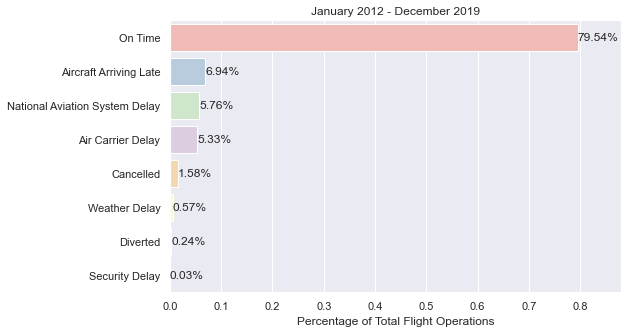
\includegraphics[width = \textwidth]{bar_plot1}
\caption{On-Time Arrival Performance By Flight Status}\label{fig:bar_plot1}
\end{figure}

Based on the bar plot, we observe that about 80\% of the flights during the eight years are on time. About 1.58\% of the flights are canceled, and about 0.24\% of them are diverted to another destination. The rest of the categories are different reasons for the delay. 

Furthermore, a lot of people are wondering about the delay rate for each year and see if improvements have been made. The bar chart in Figure \ref{fig:bar_plot2} shows that between 2012 and 2019, most delay rates are between 17\% and 22\% with the highest delay rate in 2014 and the lowest in 2016. We believe the difference of about 5\% in delay rates is significant and deserves a more thorough investigation. In general, the delay rate has not been going down.

\begin{figure}[h!]
\centering
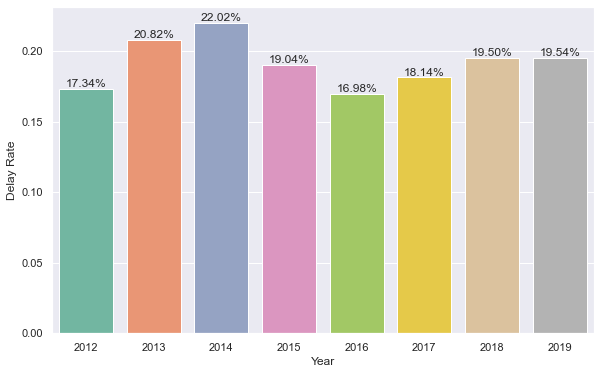
\includegraphics[width = 0.8\textwidth]{bar_plot2}
\caption{On-Time Arrival Performance By Year}\label{fig:bar_plot2}
\end{figure}

Table \ref{tab:busy} shows a numerical comparison between the less busy airports and the busiest airports on delay rates. Except for 2014, delay rates are higher for the busiest airports. The difference between the delay rates for each year is about 2 to 3 percent.

\begin{table}[h!]
\centering
\begin{tabular}{lcccccccc}
             & 2012 & 2013 & 2014 & 2015 & 2016 & 2017 & 2018 & 2019 \\ 
\hline
 Less Busy Airports & 16.97\% & 20.66\% & 22.11\% & 18.57\% & 16.19\% & 17.40\% & 18.94\% & 19.02\% \\  
 Busiest Airports & 18.39\% & 21.30\% & 21.75\% & 20.40\% & 19.16\% & 20.22\% & 20.93\% & 21.23\% \\
\end{tabular}\caption{Delay Rate for Busiest and Less Busy Airports}\label{tab:busy}
\end{table}

Last but not least, we can do a similar exploratory data analysis to compare the delay rates for national carriers and major carriers, as shown in Table \ref{tab:carrier}. The statistics appear that national carriers have a higher delay rate than major carriers (about 2\% to 3\%) for all years between 2012 and 2019. This may suggest that smaller airline companies have a higher probability of flight delay compared to larger airline carriers.

\begin{table}[h!]
\centering
\begin{tabular}{lcccccccc}
             & 2012 & 2013 & 2014 & 2015 & 2016 & 2017 & 2018 & 2019 \\ 
\hline
 National Carriers & 18.23\% & 21.95\% & 23.60\% & 21.25\% & 19.37\% & 19.91\% & 20.66\% & 20.36\% \\  
 Major Carriers & 16.97\% & 20.20\% & 21.51\% & 18.36\% & 16.12\% & 17.54\% & 18.70\% & 18.99\% \\
\end{tabular}\caption{Delay Rate for National Carriers and Major Carriers}\label{tab:carrier}
\end{table}

\bibliographystyle{abbrv}
\bibliography{refs}

\end{document}